\section{Principe.}

Ce jeu est inspiré des règles du tir à l'arc. Il y a une cible avec des cercles concentriques, correspondants chacun à un score. L'objectif est de lancer de petites billes le plus proche possible du centre afin de marquer des points.

Le robot est un adversaire mécanique pour avoir un adversaire même lorsqu'on est seul. Il se contrôle avec un smartphone android devant être équipé du bluetooth. Plus de détails sur l'application au chapitre~\ref{andro}.

\section{Déroulement d'une partie.}
\begin{enumerate}
	\item Le joueur lance l'application et se connecte au robot.
	\item Le joueur choisit le niveau de difficulté (voir section~\ref{reg_dif} un peu plus bas).
	\item Le joueur choisit le nombre de manches entre 1 et 100.
	\item Le joueur lance une bille et indique son score sur l'application.
	\item Le robot calcule la trajectoire de la bille et tire.
	\item Les dernieres manches se font de la même manière.
	\item Le smartphone affiche le score final ainsi qu'une appréciation.
\end{enumerate}

Cet enchainement est représenté par le logigramme~\ref{reg_log}.

\section{Niveaux de difficulté.} \label{reg_dif}
Il existe quatres niveaux de difficulté : \begin{description}
	\item[Facile] Le robot met majoritairement la balle sur la barre extérieure de la cible.
	\item[Moyen] Le robot met majoritairement la balle sur la barre intermédiaire de la cible.
	\item[Difficile] Le robot met majoritairement la balle au centre de la cible.
	\item[Divin] Le robot met toujours la balle au centre.
\end{description}

Même si la cible possède neuf cercles de score, ils sont découpé en trois grandes barres de trois niveau chacun pour les mesures de difficulté. Les différents niveaux sont représentés sur la figure~\ref{dif_lvl}.

Quand une des barres est majoritairement ciblé, cela signifie qu'elle totalise $\frac{3}{5}$ des tirs. Cette valeur correspond aux barres rouges sur le graphique~\ref{dif_lvl}.

\begin{figure}
	\begin{center}
		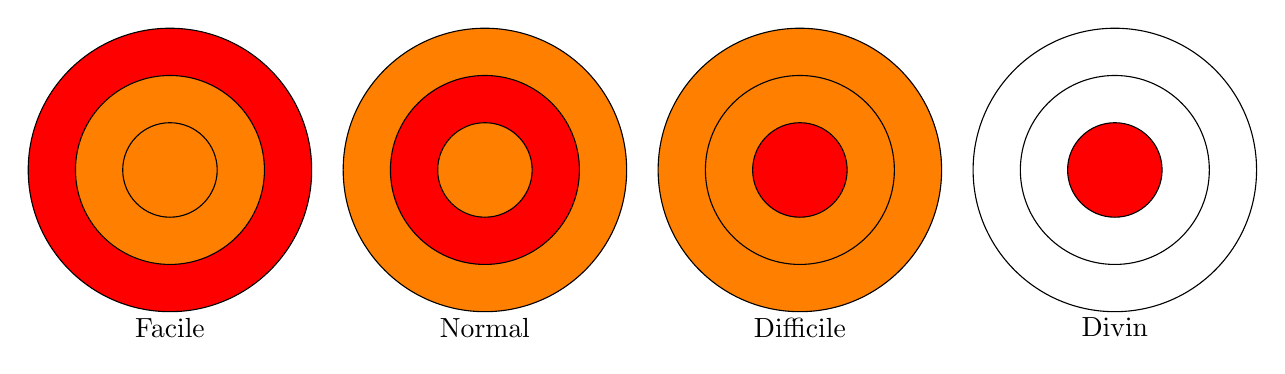
\begin{tikzpicture}
			% facile
			\filldraw[fill=red,draw=black] (-6,0) circle [radius=1.8];
			\filldraw[fill=orange,draw=black] (-6,0) circle [radius=1.2];
			\filldraw[fill=orange,draw=black] (-6,0) circle [radius=0.6];
			\draw (-6,-2) node {Facile};

			% Normal
			\filldraw[fill=orange,draw=black] (-2,0) circle [radius=1.8];
			\filldraw[fill=red,draw=black] (-2,0) circle [radius=1.2];
			\filldraw[fill=orange,draw=black] (-2,0) circle [radius=0.6];
			\draw (-2,-2) node {Normal};

			% Difficile
			\filldraw[fill=orange,draw=black] (2,0) circle [radius=1.8];
			\filldraw[fill=orange,draw=black] (2,0) circle [radius=1.2];
			\filldraw[fill=red,draw=black] (2,0) circle [radius=0.6];
			\draw (2,-2) node {Difficile};

			% Divin
			\filldraw[fill=white,draw=black] (6,0) circle [radius=1.8];
			\filldraw[fill=white,draw=black] (6,0) circle [radius=1.2];
			\filldraw[fill=red,draw=black] (6,0) circle [radius=0.6];
			\draw (6,-2) node {Divin};
		\end{tikzpicture}
	\end{center}
	\caption{Niveaux de difficulté.}
	\label{dif_lvl}
\end{figure}

\begin{figure}
	\begin{center}
		\begin{tikzpicture}[node distance=1.5cm]
			\node[entity] (first) {Connection};
			\node[weak entity] (second) [below of=first] {Difficulté} edge (first);
			\node[weak entity] (third) [below of=second] {Manches} edge (second);
			\node[relationship] (cond) [below of = third,node distance=2.5cm] {Reste manche ?} edge (third);
			\node[entity] (end) [right of=cond,node distance=3cm] {Fin} edge (cond);
			\node[entity] (joueur) [below of=cond,node distance=2.5cm] {Joueur tire} edge (cond);
			\node[entity] (ordi) [below of=joueur] {Robot tire} edge (joueur);
			\draw (0,-10) -- (0,-11);
			\draw (0,-11) -- (-3,-11);
			\draw (-3,-11) -- (-3,-5.5);
			\draw[->] (-3,-5.5) -- (-1.6,-5.5);
		\end{tikzpicture}
	\end{center}
	\caption{Déroulement d'une partie.}
	\label{reg_log}
\end{figure}


